% !Mode:: "TeX:UTF-8"
\chapter{Программная реализация}

%%\begin{abstract}
%{\textit Небольшое отступление о множествах, функциях полезности и
%прагматике. Уравнения с множествами (и вообще использование
%множеств) взялись из попытки компактного описания
%последовательностей кэш-промахов и кэш-попаданий (интересно, как с
%этой проблемой борется Genesys-Pro). Компактность удалось достичь.
%Была надежда, что эта компактная форма записи даст и неплохой
%алгоритм разрешения (с глубоким использованием особенностей операций
%над множествами). Однако на реальных данных формула, выписанная на
%множествах, получалась очень большой длины (пропорционально размеру
%самой кэш-памяти). К счастью, появилась иная идея описания
%кэш-попаданий и кэш-промахов в ограничениях -- использование функций
%полезности (т.е. ограничения вида <<тегсет еще не вытеснен/тегсет
%уже вытеснен>>). В общем случае использование функций полезности не
%дает выигрыша, но при совместном рассмотрении кэш-памяти и TLB, т.е.
%при возможности использовать пересечение хранящихся в них данных,
%удается выписать ограничения компактного размера с использованием
%функций полезности.
%
%Таким образом, в работе представлены два новых способа записи
%тестовых ситуаций в кэш-памяти с использованием ограничений --
%уравнения на множества тегов и уравнения с функциями полезности.}
%%\end{abstract}

\section{Структура генератора тестовых программ}

В главе описывается система генерации тестовых программ на основе
тестовых шаблонов. Входными данными системы являются:
\begin{itemize}
\item тестовый шаблон;
\item описания тестовых ситуаций;
\item начальное состояние микропроцессора;
\item дополнительные параметры конфигурации.
\end{itemize}

Выходом системы является тестовая программа, удовлетворяющая
тестовому шаблону с учетом данных описаний тестовых ситуаций и
начального значения микропроцессора. Ядром системы является
\emph{генератор ограничений} (см. рис.~\ref{structure}). Ограничения
разрешаются другим компонентом системы -- \emph{решателем
ограничений}. Модель, построенную решателем ограничений, анализирует
\emph{генератор инструкций тестовой программы}, с целью построить
готовую тестовую программу.

\begin{figure}[h] \center
  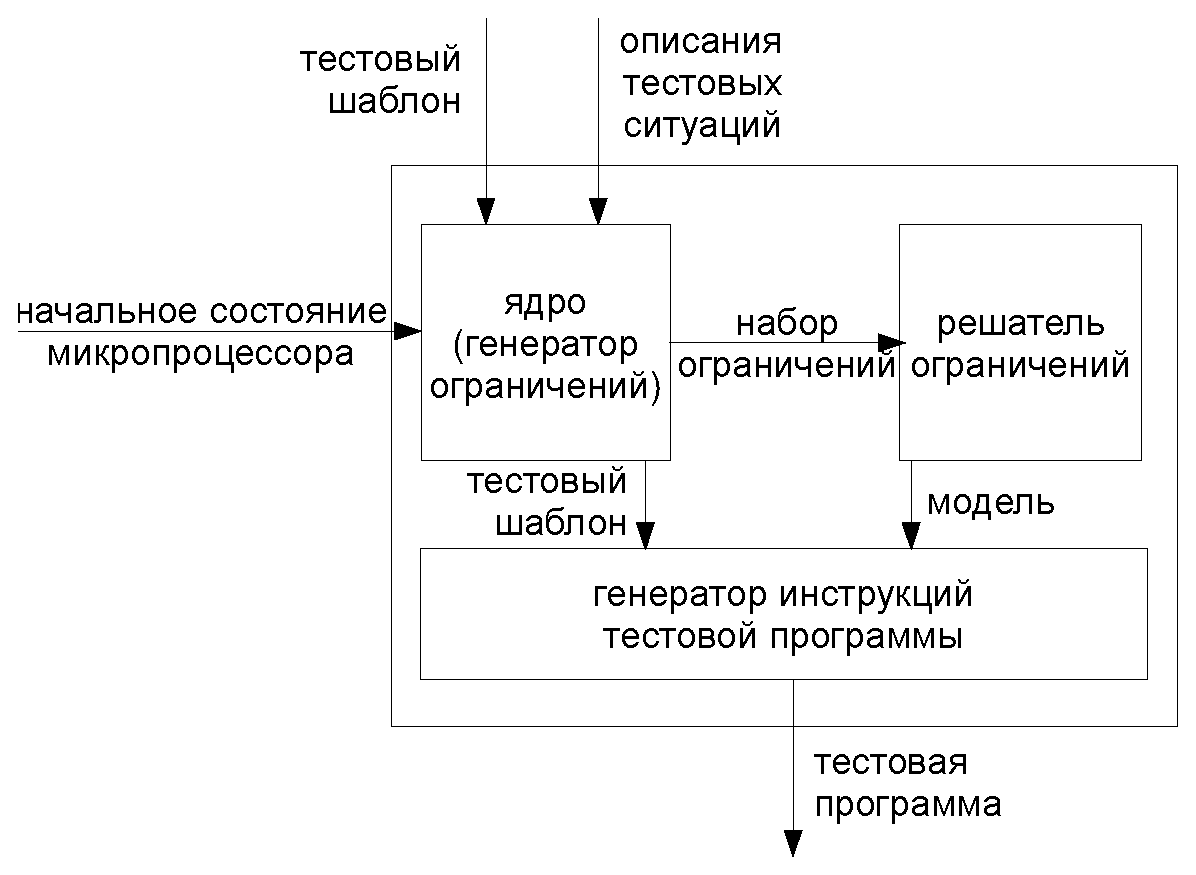
\includegraphics[width=0.8\textwidth]{3.impl/structure}\\
  \caption{Структура системы генерации тестовых программ}\label{structure}
\end{figure}

На рис.~\ref{comparison_genesyspro} показано сравнение предлагаемого
генератора тестовых программ с известным генератором
Genesys-Pro~\cite{GenesysPro}. Оба генератора получают на вход
тестовый шаблон, а на выходе у них тестовые программы.

Genesys-Pro на вход требует architectural model и testing knowledge
-- первая дает по сути эталонный симулятор микропроцессора (задает
операционную семантику инструкций и модель состояния
микропроцессора), а второй описывает эвристики выбора аргументов для
инструкции. Genesys-Pro чётко разделяет свойства аргументов
инструкции и свойства результата инструкции, соотношение между ними
задается не с помощью ограничений (т.е. не декларативным способом),
а в виде алгоритма (т.е. императивным способом). Genesys-Pro не
предполагает систематического описания семантики инструкций,
выделения ветвей их функциональности, описания программных
контрактов инструкций. Симулятор нужен для построения модельного
состояния микропроцессора после исполнения очередной сгенерированной
инструкции, а эвристики выбора аргументов составляют основу тех
ограничений, которые описывают значения аргументов очередной
инструкции.

Другой особенностью Genesys-Pro является то, что поддерживаемые им
тестовые шаблоны зачастую не фиксируют последовательность инструкций
(это позволяет строить более простые ограничения, потому как
генерируемая последовательность инструкций может по ходу генерации
подстраиваться под уже сгенерированные инструкции со
сгенерированными значениями аргументов, под состояние
микропроцессора, в которое привели сгенерированные инструкции).

Выразительный язык Genesys-Pro для описания ограничений однако
содержит такие нетривиальные конструкции, как явное использование
элементов массивов данных, что требует для разрешения продвинутый
решатель CSP, в том числе и заточенный под особенности генерации
тестовых данных для тестовых шаблонов (как минимум такие ограничения
могут включать битовые операции). Подобный решатель был разработан в
IBM для инструмента Genesys-Pro~\cite{GenesysSolver}. Однако
создание такого решателя -- отдельное сложное исследование, которое
не входило в цели данного исследования. В данной работе было принято
решение использовать доступные существующие решатели (не обязательно
CSP) и сосредоточиться на упрощении генерируемых ограничений для
некоторых частных случаев архитектур.

\begin{figure}[h]
\parbox{0.5\textwidth}{ \centering
  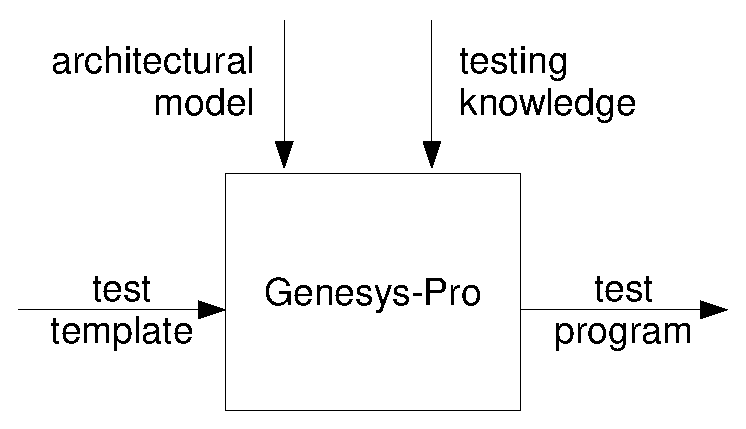
\includegraphics[width=0.45\textwidth]{3.impl/genesys-pro}
} \vline
\parbox{0.5\textwidth}{ \centering
  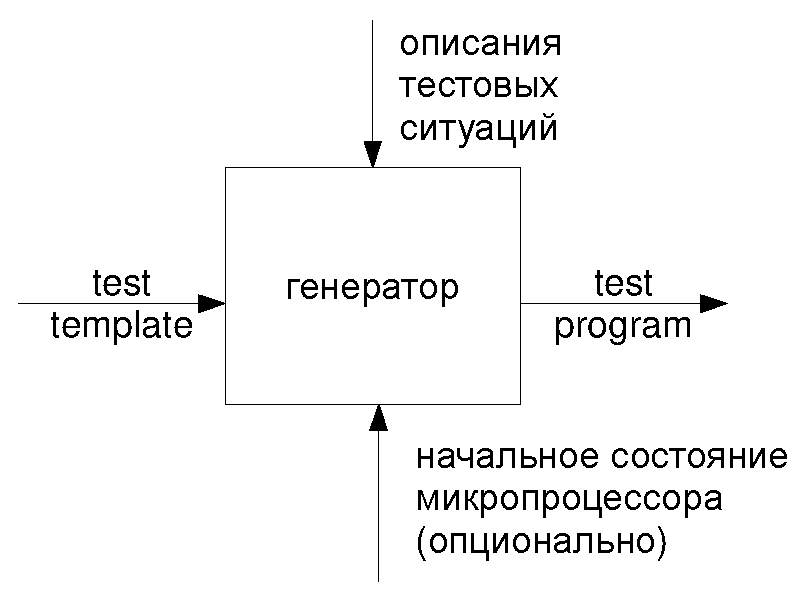
\includegraphics[width=0.45\textwidth]{3.impl/mygen}
}
\caption{Сравнение с Genesys-Pro}\label{comparison_genesyspro}
\end{figure}

В отличие от Genesys-Pro в предлагаемом инструменте описание
семантики инструкций задается в едином виде -- в виде описаний
тестовых ситуаций~\cite{my_syrcose_2008, my_isp_2008}. Каждая
тестовая ситуация описывает не только ограничение на свои аргументы,
но и результат исполнения инструкции \emph{при данном ограничении на
аргументы} инструкции декларативным образом. В функции, которую
реализует инструкция, выделяются отдельные \emph{ветви
функциональности}, ситуации различного поведения инструкций, каждая
ветвь функциональности становится отдельной тестовой ситуацией.
Например, инструкция целочисленного сложения ADD может быть
исполнена либо точно, либо с возникновением переполнения. Поэтому у
этой инструкции можно выделить 2 ветви функциональности (точное
исполнение и исполнение с переполнением), каждая ветвь дает свою
тестовую ситуацию. Кроме того, предлагаемый генератор дает
возможность указать начальное состояние микропроцессора, которое
будет эффективно использовано при построении тестовой программы.
Последовательность инструкций фиксирована и задается в тестовом
шаблоне.

Описания тестовых ситуаций можно составлять по следующей схеме:
\begin{enumerate}
\item выделить тестируемые инструкции;
\item найти описание семантики выбранных инструкций (обычно оно
входит в документацию по тестируемой архитектуре);
\item для каждой инструкции выделить:
    \begin{itemize}
    \item аргументы: имена и битовые длины;
    \item предусловие (ограничение на значения аргументов
    инструкции, при которых она может быть результативно исполнена);
    \item ветви функциональности инструкции (ситуации различного
    поведения инструкции);
    \end{itemize}
\item для каждой ветви функциональности составить описание тестовой
ситуации, поместив туда объявления аргументов, предусловие и
операторы, описывающие поведение инструкции на данной ветви
функциональности, т.е. вычисление выходного значения инструкции или
создание условий возникновения исключительной ситуации.
\end{enumerate}

Раздел~\ref{tesla} содержит описание предлагаемого языка описания
тестовых шаблонов и тестовых ситуаций, пригодный для описания
инструкций арифметической, логической подсистем, подсистемы
обращения к памяти, инструкции переходов.

\section{Описание тестовых шаблонов}\label{tesla}

Описание тестового шаблона состоит из следующих секций:
\begin{enumerate}
\item \emph{заголовок шаблона}: объявление регистров и констант;
\item \emph{тело шаблона}: инструкции и ограничения тестового
шаблона.
\end{enumerate}

Заголовок шаблона должен содержать объявления всех задействованных в
тестовом шаблоне регистров (для каждого регистра указывается его имя
и битовая длина) и констант (или по-другому, <<непосредственных
значений>> -- для каждой константы так же указывается ее имя и
битовая длина). Регистр может использоваться в качестве
аргумента-результата инструкции, константа не может использоваться в
качестве аргумента-результата инструкции. Регистры и константы
сохраняют свою битовую длину на протяжении всего тестового шаблона.
Генератор ограничений трактует регистр как переменную со значением и
генерирует начальное значение такой переменной, при которой
выполнены все заявленные в тестовом шаблоне тестовые ситуации.
Обычно для инициализации регистра достаточно одной-двух инструкций
(это зависит от количества бит, которое может изменить одна
инструкция). Константа трактуется как значение, которое не меняется.
Для нее тоже генерируется значение и при составлении тестовой
программы оно вставляется непосредственно на место аргумента
инструкций.

Пример объявления регистра и константы: {\small \begin{verbatim}
    <register id="z" length="64" />
    <constant id="c" length="16" />
\end{verbatim}}

Тело тестового шаблона состоит из описаний инструкций и ограничений.
Для инструкции необходимо указать:
\begin{itemize}
\item имя инструкции;
\item аргументы инструкции (объявленные ранее регистры или
константы);
\item внешние переменные инструкции;
\item тестовую ситуацию.
\end{itemize}

Тестовые ситуации на косвенные обращения не рассматриваются, поэтому
в описания тестовых шаблонов не включены механизмы описания
косвенных обращений.

\emph{Механизм внешних переменных} инструкции позволяет
формулировать ограничения на локальные переменные, определенные в
разных тестовых ситуациях. При объявлении новой локальной переменной
кроме имени можно указать идентификатор (имя надо указывать
обязательно, а идентификатор -- необязательно). Все идентификаторы
внутри тестовой ситуации должны быть уникальными. Это может быть
виртуальный адрес, физический адрес, некое внутреннее выражение.
Если тестовая ситуация является составной, то все тестовые ситуации
должны определять выносимые на уровень тестового шаблона
идентификаторы. На уровне тестового шаблона идентификатору ставится
в соответствие некоторое новое уникальное внутри шаблона имя,
которое можно использовать наравне с другими переменными (регистрами
или константами).

Тестовая ситуация описывает некоторое поведение инструкции. Обычно
можно выделить два типа поведений инструкции: существенное
исполнение (вычисление значения, осуществление взаимодействия) и
генерация исключения. При существенном исполнении тестовая ситуация
описывает предусловие инструкции и набор условий и вычислений,
определяющих данное поведение инструкции. При исполнении с
генерацией исключения описывается предусловие инструкции и набор
условий и вычислений, приводящих к возникновению исключения. Само
возникновение исключения, как оператор, не описывается.

Тестовая ситуация состоит из набора \emph{ветвей} -- простейших
поведений инструкции. Ветви могут \emph{комбинироваться} в
дизъюнкции и конъюнкции. Дизъюнкция ветвей (или их комбинаций)
означает, что в данный момент инструкция может себя вести согласно
хотя бы одной из ветвей. Конъюнкция ветвей (или их комбинаций)
означает, что в данный момент инструкция может себя вести согласно
всем ветвям одновременно. Объединенные в конъюнкцию ветви не могут
иметь существенное исполнение.

Пример тестовой ситуации ветви: {\small
\begin{verbatim}
        <situation>
            <branch name="overflow" />
        </situation>
\end{verbatim}}

Для ветви указывается имя. Оно используется при поиске
соответствующего файла с описанием этой тестовой ситуации. Поиск
производится на основе имени тестовой ситуации и имени инструкции,
для которой она указана.

Пример тестовой ситуации, включающей комбинацию ветвей: {\small
\begin{verbatim}
        <situation>
            <or>
                <and>
                    <branch name="overflow" />
                    <branch name="normal" />
                </and>
                <branch name="zero" />
            </or>
        </situation>
\end{verbatim}}

Эту комбинацию ветвей можно прочесть следующим образом: \emph{данная
инструкция должна себя вести как overflow с normal или как zero}.

В описаниях тестовых ситуациях могут быть фиксированы обращения к
различным подсистемам микропроцессора. Указание тестовой ситуации в
шаблоне может фиксировать и тестовую ситуацию на эти обращения (а
для полных тестовых шаблонов оно \emph{должно} фиксировать тестовую
ситуацию на эти обращения). Среди подсистем можно выделить различные
кэширующие буферы (например, уровни кэш-памяти, TLB, другие
подсистемы). Содержимое секции тестовых ситуаций обращений к
подсистемам определяется архитектурой тестируемого микропроцессора.
Например, оно может быть следующим: {\small
\begin{verbatim}
    <situation>
            ...
            <access>
                <cache level="1" type="DATA" id="miss" />
                <cache level="2" type="DATA" id="miss" />
                <cache level="3" type="DATA" id="hit" />
                <tlb  id="invalid">
                    <microtlb type="DATA" id="miss" />
                </tlb>
            </access>
    </situation>
\end{verbatim}}

Это описание говорит о том, что при исполнении данной инструкции в
кэш-памяти данных первого и второго уровней должен быть кэш-промах,
а в кэш-памяти данных третьего уровня -- кэш-попадание; в TLB должна
произойти тестовая ситуация invalid, а в MicroTLB данных -- промах.
Интерпретация терминов \texttt{cache, tlb, microtlb, miss, hit,
invalid} заложена в части генератора ограничений, ответственного за
тестируемую архитектуру.

Кроме инструкций тестовый шаблон может содержать <<допущения>>
(assume) -- некоторые ограничения на текущее состояние
микропроцессора и введенные внешние переменные. Можно выделить
следующие основные применения этих ограничений:
\begin{enumerate}
\item задание зависимостей на адреса разных инструкций (например, у
двух инструкций одинаковые физические адреса при разных виртуальных
адресах -- одна инструкция определяет свои виртуальный и физический
адрес, другая инструкция делает то же, а ограничение фиксирует связь
значений этих четырех переменных);
\item задание ветви в графе потока управления: при тестировании
инструкций перехода с некоторым сравнением вместо их
непосредственного описания предлагается описывать конкретные
результаты сравнений (истинно это сравнение в данный момент или
ложно); тестовый шаблон не позволяет описывать разветвленные потоки
управления, разрешается описывать лишь последовательности
инструкций, поэтому такие дополнительные ограничения позволяют
описать в тестовом шаблоне один из путей в графе потока управления и
сгенерировать для этого пути свою тестовую программу.
\end{enumerate}

Описание ограничения, как и описание тестовой ситуации, может
состоять из указания ветви или их комбинаций. Пример: {\small
\begin{verbatim}
    <assume>
        <or>
            <and>
                <branch name="ff1" />
                <branch name="ff2" />
                <branch name="ff3" />
            </and>
            <branch name="ff4" />
        </or>
    </assume>
\end{verbatim}}

Пример описания тестового шаблона целиком: {\small
\begin{verbatim}
  <template>
    <register id="x" length="64" />
    <register id="y" length="64" />
    <register id="z" length="64" />
    <constant id="c" length="16" />

    <instruction name="ADD">
        <argument name="x" />
        <argument name="y" />
        <argument name="z" />
        <external name="v1" id="virtual" />
        <external name="p1" id="phys" />
        <situation>
            <or>
                <and>
                    <branch name="overflow" />
                    <branch name="normal" />
                </and>
                <branch name="zero" />
            </or>

            <access>
                <cache level="1" type="DATA" id="miss" />
                <cache level="2" type="DATA" id="miss" />
                <cache level="3" type="DATA" id="hit" />
                <tlb  id="invalid">
                    <microtlb type="DATA" id="miss"></microtlb>
                </tlb>
            </access>

        </situation>
    </instruction>

    <assume>
        <or>
            <and>
                <branch name="ff1" />
                <branch name="ff2" />
                <branch name="ff3" />
            </and>
            <branch name="ff4" />
        </or>
    </assume>
</template>
\end{verbatim}
 }

\section{Описание тестовых ситуаций}

Описание тестовой ситуации состоит из следующих секций:
\begin{enumerate}
\item \emph{заголовок тестовой ситуации}: объявление аргументов инструкции;
\item \emph{тело тестовой ситуации}: последовательность операторов.
\end{enumerate}

Заголовок тестовой ситуации должен содержать объявления всех
аргументов инструкции. Для каждого аргумента указывается его имя
(локальное внутри данной тестовой ситуации), статус <<только для
чтения/результат>> и битовая длина. Последовательность аргументов
тестовой ситуации должна совпадать с последовательностью аргументов
инструкции с точностью до переименования. Иными словами, первый
аргумент тестовой ситуации должен обозначать первый аргумент
инструкции (их битовые длины должны совпадать), второй аргумент
тестовой ситуации -- второй аргумент инструкции и так далее.
Аргументы, помеченные статусом <<только для чтения>> не могут менять
свое значение во время всей тестовой ситуации. Аргументы, помеченные
статусом <<результат>> обязаны получить значение в данной
инструкции. Тестовая ситуация может иметь произвольное количество
аргументов обоих статусов в произвольном порядке. Статус <<только
для чтения>> позволяет передать в качестве аргументов инструкции
одинаковые переменные (одинаковые регистры или константы). Однако
все аргументы инструкции, соответствующие аргументам тестовой
ситуации со статусом <<результат>>, должны иметь разные имена (они
могут быть среди аргументов со статусом <<только для чтения>>).

Пример: {\small
\begin{verbatim}
 <argument name="rt" state="result" length="64"/>
 <argument name="base" state="readonly" length="64"/>
 <argument name="offset" state="readonly" length="16"/>
\end{verbatim}}

Тело тестовой ситуации состоит из последовательности операторов трех
видов:
\begin{itemize}
  \item оператор \texttt{let} -- объявление новой локальной
  переменной вместе с ее инициализацией;
  \item оператор \texttt{assume} -- фиксация некоторого ограничения
  (<<допущения>>) на значения переменных;
  \item оператор \texttt{procedure} -- вызов процедуры (ее семантика
    не задается в описании тестовой ситуации).
\end{itemize}

Тестовая ситуация по своей сути является ветвью функциональности
инструкции. Поэтому ее описание содержит лишь последовательность
операторов, условные операторы и операторы цикла отсутствуют.

Оператор \texttt{let} объявляет новую переменную и инициализирует ее
результатом вычисления некоторого выражения. Оператор может
содержать указание имени переменной (оно должно быть новым)
\emph{или} указание идентификатора новой переменной (все
идентификаторы внутри тестовой ситуации должны быть разными;
идентификатор может совпадать с именем этой или любой другой
переменной). Безымянные операторы \texttt{let} позволяют задать
идентификатор существующей переменной.

Тело оператора содержит выражение, результат вычисления которого
станет значением объявляемой переменной. Выражение может содержать
следующие операции:
\begin{itemize}
  \item переменные (\texttt{var}) и константы (\texttt{constant});
  допустимы только неотрицательные константы, у каждой константы
  должна быть указана битовая длина;
  \item битовые операции: выделение бита с заданными номером (\texttt{bit}),
  выделение непрерывной последовательности бит с заданными границами
  (\texttt{bits}), битовая конкатенация (\texttt{concat}), битовая
  степень (\texttt{power});
  \item арифметические операции: сложение (\texttt{sum}), вычитание
  (\texttt{sub}); операции проводятся по модулю экспоненты битовой
  длины аргументов.
\end{itemize}
Производится строгая <<проверка типов>>, т.е. битовых длин
аргументов операций. Например, сложению подвергаются только
выражения с одинаковыми битовыми длинами. В частности это позволяет
автоматически вычислить битовую длину объявляемой переменной.

Пример: {\small
\begin{verbatim}
<let name="vAddr" id="virtual">
    <sum>
        <sign_extend size="64"><var>offset</var></sign_extend>
        <var>base</var>
    </sum>
</let>
\end{verbatim}}

Оператор \texttt{assume} позволяет указать ограничение, справедливое
в некоторый момент на значениях аргументов тестовой ситуации и
локальных переменных. Выражения объединяются с помощью отношений
сравнения. Пример: {\small
\begin{verbatim}
    <assume>
        <eq>
            <bits end="1" start="0"><var>vAddr</var></bits>
            <constant length="2">0</constant>
        </eq>
    </assume>
\end{verbatim}}

Оператор \texttt{procedure} позволяет указать более сложное
действие, в котором могут участвовать различные подсистемы
микропроцессора. Семантика процедур не фиксируется при описании
тестовой ситуации. Аргументы, наоборот, фиксируются. Каждый аргумент
может иметь идентификатор (это позволяет располагать аргументы в
произвольном порядке, указывая семантику каждого аргумента с помощью
идентификатора). Тело аргумента может быть следующих типов:
\begin{itemize}
  \item выражение на определенные к моменту вызова процедуры
  переменные; выражение задается с использованием того же
  синтаксиса, что и в операторе \texttt{let};
  \item новая переменная (\texttt{new});
  \item символьная константа.
\end{itemize}

Набор допустимых процедур и идентификаторов их аргументов задается
генератором ограничений.

Пример: {\small
\begin{verbatim}
<procedure name="AddressTranslation">
        <argument id="physical"><new length="64">pAddr</argument>
        <argument id="virtual"><var>vAddr</var></argument>
        <argument id="points_to">DATA</argument>
        <argument id="points_for">LOAD</argument>
</procedure>
\end{verbatim}}

Пример описания тестовой ситуации целиком: {\small
\begin{verbatim}
<situation>
    <argument name="rt" state="result" length="64" />
    <argument name="base" state="readonly" length="64" />
    <argument name="offset" state="readonly" length="16" />

    <let name="vAddr" id="virtual">
        <sum>
            <sign_extend size="64"><var>offset</var></sign_extend>
            <var>base</var>
        </sum>
    </let>

    <assume>
        <eq>
            <bits end="1" start="0"><var>vAddr</var></bits>
            <constant length="2">0</constant>
        </eq>
    </assume>

    <procedure name="AddressTranslation">
        <argument id="physical"><new length="64">pAddr</argument>
        <argument id="virtual"><var>vAddr</var></argument>
        <argument id="points_to">DATA</argument>
        <argument id="points_for">LOAD</argument>
    </procedure>

    <let id="physical"><var>pAddr</var></let>

    <let name="dwByteOffset">
        <bits end="2" start="0"><var>vAddr</var></bits>
    </let>

    <!-- dwByteOffset can be changed
         according to BigEndian/LittleEndian -->

    <procedure name="LoadMemory">
        <argument id="data"><new length="64">memdoubleword</argument>
        <argument id="size">WORD</argument>
        <argument id="physical"><var>pAddr</var></argument>
        <argument id="virtual"><var>vAddr</var></argument>
        <argument id="points_to">DATA</argument>
    </procedure>

    <procedure name="BytesSelect">
        <argument id="type">WORD</argument>
        <argument id="from"><new length="32">data</argument>
        <argument id="content"><var>memdoubleword</var></arument>
        <argument id="index"><var>dwByteOffset</var></argument>
    </procedure>

    <assume>
        <eq>
            <var>rt</var>
            <sign_extend size="64"><var>data</var></sign_extend>
        </eq>
    </assume>
</situation>
\end{verbatim}}

\section{Генератор ограничений (ядро)}

Генератор ограничений имеет модульную структуру (см.
рис.~\ref{generator})~\cite{my_lomonosov_2009, my_miet_2009}. В его
составе есть модуль, ответственный за генерацию ограничений для
общих механизмов описания архитектур микропроцессоров, такие как
работа с регистрами, работа с последовательностью инструкций, работа
с локальными переменными в тестовых ситуаций, и модуль, специфичный
для тестируемой архитектуры (он содержит алгоритмы генерации
ограничений для таких механизмов, как трансляция адресов, как
кэширование).

\begin{figure}[h] \center
  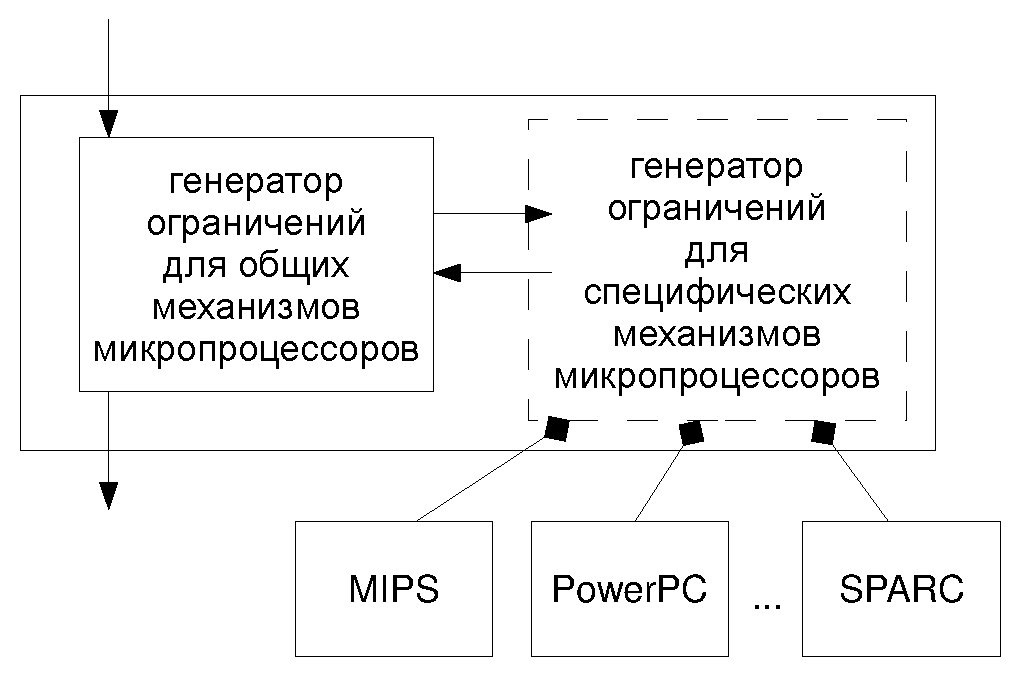
\includegraphics[width=0.5\textwidth]{3.impl/generator}\\
  \caption{Структура генератора ограничений}\label{generator}
\end{figure}

Генерация ограничений производится последовательно для каждой
инструкции тестового шаблона. Однако разрешение ограничений может
происходить быстрее при некотором порядке ограничений, это можно
учесть при генерации ограничений.
